
\title{T-61.5130 Machine Learning and Neural Networks}
\author{Karhunen, Luttinen}
\date{Exercise 11, ??.??.2012}

\newcommand{\vect}[1]{{\bf{#1}}}
\newcommand{\svect}[1]{\boldsymbol{#1}}
\newcommand{\matr}[1]{\boldsymbol{#1}}


\begin{document}

\maketitle

\begin{enumerate}

\item In this problem we consider the optimized form of the learning
  vector quantization algorithm developed by
  Kohonen. We wish to arrange for the effects of the corrections to the
  Voronoi vectors, made at different times, to have equal influence when
  referring to the end of the learning period. \begin{enumerate}
  \item First, show that
    \begin{equation}
      \mathbf{w}_c(n+1)=\mathbf{w}_c(n)+\alpha_n[\mathbf{x}_i-\mathbf{w}_c(n)]
      \label{equation: 1}
    \end{equation}
    and
    \begin{equation}
      \mathbf{w}_c(n+1)=\mathbf{w}_c(n)-\alpha_n[\mathbf{x}_i-\mathbf{w}_c(n)]
      \label{equation: 2}
    \end{equation}
    may be integrated into a single equation, as follows:
    \begin{equation}
      \mathbf{w}_c(n+1)=(1-s_n\alpha_n)\mathbf{w}_c(n)+s_n\alpha_n\mathbf{x}(n).
      \label{equation: 3}
    \end{equation}
    In the above equations, $\mathbf{w}_c$ is the Voronoi
    vector closest to the input vector $\mathbf{x}_i$, $0<\alpha_n<1$ is a
    learning constant, and $s_n$ is a sign function depending on the
    classification result of the $n$th input vector $\mathbf{x}(n)$:
    $s_n=+1$ if classification is correct, otherwise  $s_n=-1$.

  \item Hence, show that the optimization criterion described at the
    beginning of the problem is satisfied if
    \begin{equation*}
      \alpha_n=(1-s_n\alpha_n)\alpha_{n-1}
    \end{equation*}
    which yields the optimized value of the learning constant
    $\alpha_n$ as
    \begin{equation*}
      \alpha_n^{\text{opt}}=\frac{\alpha_{n-1}^{\text{opt}}}{1+s_n\alpha_{n-1}^{\text{opt}}}.
    \end{equation*}
  \end{enumerate}

  \begin{solution}
    
    Part a) is seen by inserting $s_n=1$ and $s_n=-1$ into equation (\ref{equation: 3}) yielding the two
    update equations (\ref{equation: 1}) and (\ref{equation: 2}).

    For the LVQ equation we note that the updated weight vector
    $\mathbf{w}_c(n+1)$ contains a ``trace'' from  $\mathbf{x}(n)$ by
    virtue of the last term $s_n\alpha_n\mathbf{x}(n)$. Moreover, it
    contains traces of previous samples, namely, $\mathbf{x}(n-1)$,
    $\mathbf{x}(n-2),\;\ldots,\; \mathbf{x}(1)$ by virtue of the present
    value of the weight vector $\mathbf{w}_c(n)$.

    Consider $\mathbf{w}_c(n)$ which is defined by
    \begin{equation}
      \mathbf{w}_c(n)=(1-s_{n-1}\alpha_{n-1})\mathbf{w}_c(n-1)+s_{n-1}\alpha_{n-1}\mathbf{x}(n-1)
      \label{eq:lvq2}
    \end{equation}
    Hence, substituting equation \ref{eq:lvq2} into the LVQ equation and
    combining terms yields
    \begin{equation}
      \mathbf{w}_c(n+1)=(1-s_n\alpha_n)(1-s_{n-1}\alpha_{n-1})\mathbf{w}_c(n-1)+(1-s_n\alpha_n)s_{n-1}\alpha_{n-1}\mathbf{x}(n-1)+s_n\alpha_n\mathbf{x}(n).
      \label{eq:lvq3}
    \end{equation}
    It follows therefore that the effect of $\mathbf{x}(n-1)$ on the
    updated weight vector $\mathbf{w}_c(n+1)$ is scaled by the factor
    $(1-s_n\alpha_n) s_{n-1} \alpha_{n-1}$. On the other hand, the effect of
    $\mathbf{x}(n)$ is scaled by $s_n\alpha_n$. Accordingly, if we require
    that $\mathbf{x}(n)$ and $\mathbf{x}(n-1)$ are to have the same effect
    on $\mathbf{w}_c(n+1)$, then we must have
    \begin{equation*}
      | s_n \alpha_n |= | (1-s_n\alpha_n)\alpha_{n-1} s_{n-1} |.
    \end{equation*}
    Since $s_{n-1}$ and $s_n$ are either $1$ or $-1$, their absolute values are $1$. The remaining quantities inside
    the absolute values are positive and we obtain
    \begin{equation*}
      \alpha_n = (1-s_n\alpha_n)\alpha_{n-1} .
    \end{equation*}

    Solving for $\alpha_n$, we get the optimum
    \begin{equation*}
      \alpha_n^{opt}=\frac{\alpha_{n-1}^{opt}}{1+s_n\alpha_{n-1}^{opt}}.
    \end{equation*}



  \end{solution}
  

\item Using the LMS algorithm, formulate a learning algorithm for the
  focused neuronal filter.


  \begin{solution}

    The neuronal filter is a block which is drawn in the figure:
    % 
    % \begin{figure}
    %   \centering
    %   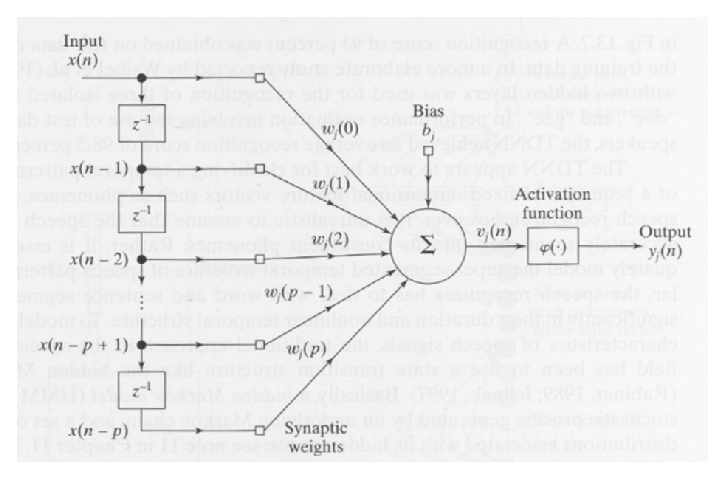
\includegraphics[width=11cm]{l12k3a.eps} 
    %   \label{figure: 1}
    % \end{figure}
    % 

    % \hspace{2cm}
    \begin{center}
      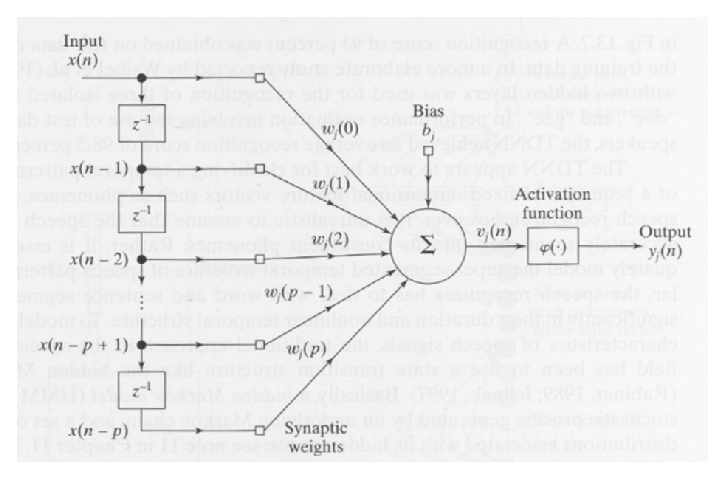
\includegraphics[width=11cm]{l12k3a.eps}
    \end{center}

    % 
    The output of the filter is $y(n) =
    \varphi(v(n))$, where $v(n)$ is the linear response of the neuron $$v(n) = b +
    \sum_{l=0}^p w(l) x(n-l) \, .$$ (Notice that for convenience we use
    a simpler notation, where the index of the neuron is dropped.)
    The least mean square (LMS) algorithm aims at minimising the mean
    square error $$\mathcal{E} = \sum_n \mathcal{E}(n) = \frac{1}{2} \sum_n e(n)^2 \, ,$$
    where $e(n) = d(n) - y(n)$ is the error made by the network.  For deriving an
    on-line learning algorithm we  use the stochastic
    gradient descent method where one proceeds in the direction of the negative
    gradient of the instantaneous
    error $\mathcal{E}(n)$.

    From the chain rule we have $$\frac{\partial \mathcal{E}(n)}{\partial w(l)} =
    \frac{\partial \mathcal{E}(n)}{\partial e(n)} \frac{\partial e(n)}{\partial
      y(n)} \frac{\partial y(n)}{\partial v(n)} \frac{\partial
      v(n)}{\partial w(l)} = e(n) (-1) \varphi'(v(n)) x(n-l) \, .$$ 
    $\varphi'$ denotes the derivative of the activation function.
    The
    learning rule for adjusting the weight $w_l$ is thus $\Delta w_l = -\eta \partial \mathcal{E}(n) / \partial
    w(l) = \eta e(n) \varphi'(v(n)) x(n-l)$, where $\eta$ is the learning
    rate.  A similar derivation for the bias $b$ will give the learning
    rule $\Delta b = - \eta \partial \mathcal{E}(n) / \partial b = \eta e(n)
    \varphi'(v(n))$.
    % }

  \end{solution}
  
\item How would you design a tapped delay line for a focused time
  lagged feedforward network?


  \begin{solution}

    Once the structure is fixed, the parameters can be learned for
    instance by temporal back-propagation.  For the design of the structure there are no
    general rules.  Cross-validation, Bayesian models selection etc.
    can be used but the structure of the delay line has very many
    degrees of freedom.

    The available prior knowledge about the plausible time lags should
    be used for choosing the lengths of the delays, possible averaging
    lengths and so on.  Often it is reasonable to have a higher
    resolution for the immediate past and increasingly coarse
    resolution for more distant past.


  \end{solution}
  
\item Discuss how the temporal back-propagation algorithm may be used for the
  training of a distributed time lagged feedforward network (TLFN) for single-step prediction.

  \begin{solution}

    Let $\mathbf{x}(n)=[x(n), x(n-1), \ldots ,x(n-p)]$ denote the vector of current and
    delayed input signals applied to
    the distributed TLFN at time $n$. Let $y(n)$ denote the actual
    response of the network trained using the temporal back-propagation
    algorithm. With one-step prediction as the requirement, the desired
    response is the value of the input signal one step into the future,
    that is, $x(n+1)$. With these provisions, we may then
    proceed with the temporal back-propagation algorithm.

  \end{solution}
  


\item Write out the state-space model for the recurrent network shown in the
  figure.

  \hspace{2cm}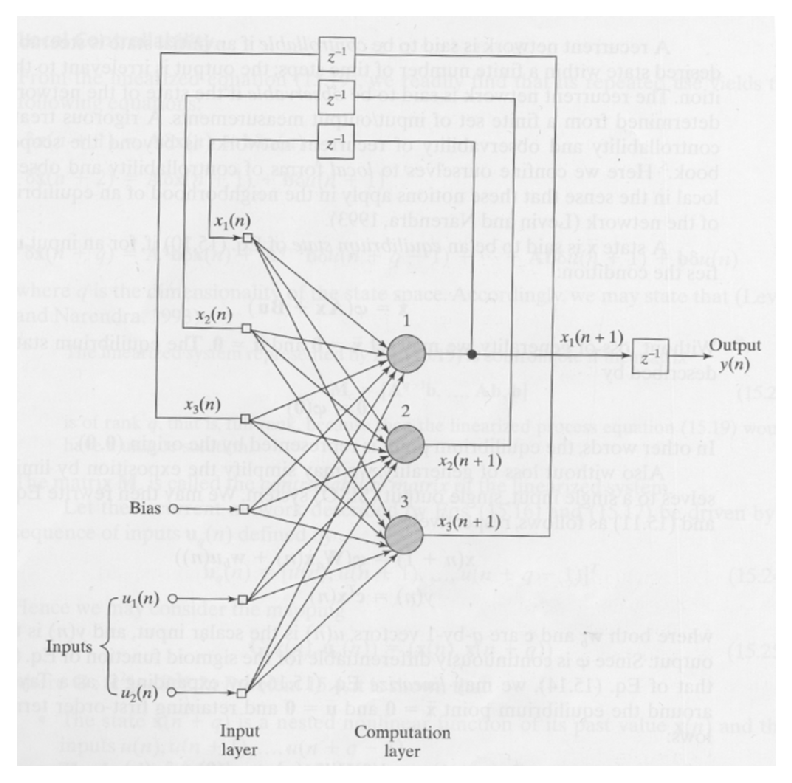
\includegraphics[width=11cm]{l12k9.eps}

  \begin{solution}

    In the figure, there are two neurons in the input layer, three neurons in the hidden layer and one
    output. In the following, we consider a more general case with arbitrary number of neurons in each layer.

    Let the $q$-by-$1$ vector $x(n)$ denote the state vector of recurrent network. Let the $m$-by-$1$ vector $\vect{u}(n)$ 
    denote the input
    applied to the system, and the $p$-by-$1$ vector $\vect{y}(n)$ denote the
    corresponding output of the system. In mathematical terms, the dynamic
    behavior of the system, assumed to be noise free, is described by the
    following pair of nonlinear equations:

    \[
    \vect{x}(n+1) = \phi (\matr{W}_a \vect{x}(n) + \matr{W}_b \vect{u}(n))
    \]

    \[
    \vect{y}(n) = \matr{C} \vect{x}(n)
    \]
    where $\matr{W}_a$ is a $q$-by-$q$ matrix, $\matr{W}_b$ is a $q$-by-($m+1$) matrix, $\matr{C}$ is a
    $p$-by-$q$ matrix and $\phi: \mathbb{R}^q \rightarrow \mathbb{R}^q$ is a
    diagonal map described by

    \[
    \phi:
    \left[\begin{array}{c}
        x_1 \\
        x_2 \\
        \vdots \\
        x_q
      \end{array}\right]
    \rightarrow
    \left[\begin{array}{c}
        \phi(x_1) \\
        \phi(x_2) \\
        \vdots \\
        \phi(x_q)
      \end{array}\right]
    \]
    for some memoryless, component-wise nonlinearity $\phi: \mathbb{R}^m$,
    $\mathbb{R}^n$, and $\mathbb{R}^p$ are called the input space, state
    space, and output space, respectively.

    In the network of the figure we have $m$=2, $q$=3 and $p$=1. Thus the
    matrices $\matr{W}$ are defined as follows

    \[
    \matr{W}_a = 
    \left[\begin{array}{ccc}
        w_{11} & w_{12} & w_{13} \\
        w_{21} & w_{22} & w_{23} \\
        w_{31} & w_{32} & w_{33} \\
      \end{array}\right]
    \]

    \[
    \matr{W}_b = 
    \left[\begin{array}{ccc}
        b_{1} & w_{14} & w_{15} \\
        b_{2} & w_{24} & w_{25} \\
        b_{3} & w_{34} & w_{35} \\
      \end{array}\right]
    \]

    where the first column of $\matr{W}_b$ represents the bias terms applied to
    neurons 1, 2 and 3. The matrix $\matr{C}$ is defined by

    \[
    \matr{C} = [1, \; 0, \; 0]
    \]

  \end{solution}

\end{enumerate}
\end{document}             % End of document.

%%% Local Variables: 
%%% mode: latex
%%% TeX-master: "ex11_solutions"
%%% End: 
